\section{Experimental Results}
\label{sec:experiments}

\subsection{Experimental design and evaluation protocol}
The experiments address two questions: whether the selected detection pipelines
provide complementary predictions on dense PCB images, and whether the proposed
training recipes improve upon controls trained on the available original-label
RF100 PCB exports. The results are separated by dataset, input resolution and
training recipe. Scores obtained from corrected labels or 1280-pixel inputs are
not compared directly with a publication using different annotations and
640-pixel inputs.

\paragraph{Native-resolution checkpoint audit.}
Four selected single-model checkpoints and two fixed weighted box fusion (WBF)
configurations are evaluated on 44 legacy test exports containing 4,905 component
boxes. These exports represent 22 filename-based board-view groups, rather than
44 independent physical boards. The models are YOLOv12s, a crop-trained YOLO26s
specialist, YOLO26s with AGWD and Squared-Dice, and PhysOT-YOLO26s. This is a
retrospective comparison of exact saved checkpoints, not a three-seed estimate
of each architecture. Subsequent annotation review found class inconsistencies
and shared photographs across splits; the measurements therefore describe the
legacy benchmark and do not establish independent-board generalization.

\paragraph{Original-label paper-dataset study.}
The second study uses the available RF100 Printed Circuit Board version-3
exports~\cite{rf100pcb}, retaining the inherited split: 543 training, 77 validation
and 41 test images. Original IDs 2, 4, 7 and 9 are remapped to four contiguous
classes without importing the reviewed annotations or the extra capacitor-name
merge. Six methods are trained with seeds 0, 1 and 2, general COCO-pretrained
initialization, and validation-selected checkpoints. This gives 18 completed
runs. The full-board arms use 100 epochs; the crop arm uses 543 full images and
543 training-only crops, with 320- and 480-pixel crop sizes and 50 epochs.
Approximately 3,400 optimizer batches are budgeted per run. Validation and test
images are not cropped. Standard online training augmentation is shared; no
offline capacitor copy-paste is added in this study.

\begin{table}[!t]
\centering\caption{Shared settings for the original-label 640-pixel study. Timing settings also apply to the native checkpoint audit.}
\label{tab:settings}\small\setlength{\tabcolsep}{4pt}
\begin{tabular}{ll}\toprule
Parameter & Setting\\\midrule
Optimizer & SGD\\
Learning rate / momentum & 0.01 / 0.937\\
Weight decay & 0.0005\\
Training batch / nominal batch & 16 / 16\\
Full-board / mixed-crop epochs & 100 / 50\\
Seeds & 0, 1, 2\\
Inference precision / batch & FP32 / 1\\
Prediction confidence floor & 0.001\\
NMS IoU, where applicable & 0.50\\
Maximum detections per image & 1,000\\
Timing hardware & NVIDIA H100 80GB\\
Warmup / measured predictions & 30 / 100\\\bottomrule
\end{tabular}\end{table}

\paragraph{Accuracy metrics.}
Both completed evaluations use the same class-aware 101-point AP implementation.
$\mathrm{mAP}_{50}$ averages the four class AP values at matching IoU 0.50;
$\mathrm{mAP}_{50:95}$ averages thresholds from 0.50 to 0.95 in steps of 0.05.
Operating precision, recall and F1 pool class-wise TP, FP and FN at confidence
0.25 and matching IoU 0.50. They are therefore fixed-operating-point statistics,
whereas AP summarizes the confidence-ranked predictions. These two forms of
measurement should not be interpreted as interchangeable.

\paragraph{Inference and timing.}
The native audit uses square 1280-pixel letterboxing, FP32, batch one and NMS
IoU 0.45 where applicable; end-to-end heads retain their native postprocessing.
WBF uses merge IoU 0.50. The two-model weights are $(1.3,1.2)$ for YOLOv12s and
the crop specialist; the four-model weights are $(1.3,1.2,1.1,1.0)$ after adding
AGWD--Squared-Dice and PhysOT. Member confidence filtering uses 0.001; rescaled
WBF scores are retained for AP. Latency includes preprocessing, model inference,
postprocessing and fusion where applicable. Disk decoding and model loading are
excluded. FPS is 1,000 divided by mean latency in milliseconds. Parameter counts
refer to stored unfused checkpoints and are summed for ensembles.

\subsection{Best single models and ensemble performance}
\begin{table*}[!t]
\centering
\caption{Retrospective results on 44 legacy native-resolution exports. Accuracy
entries are percentages; P/R/F1 pool counts at confidence 0.25 and matching IoU
0.50. Latency includes the complete prediction pipeline and WBF. Parameter
counts are stored unfused values. These are selected checkpoints, not seed averages.}
\label{tab:native}
\small\setlength{\tabcolsep}{4pt}
\begin{tabular}{lrrrrrrrr}
\toprule
Configuration & $\mathrm{mAP}_{50}$ & $\mathrm{mAP}_{50:95}$ & P & R & F1
& ms & FPS & Params (M)\\
\midrule
YOLOv12s & 66.16 & 45.45 & 61.70 & 49.42 & 54.88 & 14.33 & 69.79 & 9.25 \\
Crop-trained YOLO26s & 66.56 & 45.48 & 54.61 & 51.23 & 52.87 & 11.11 & 89.99 & 9.95 \\
AGWD + Squared-Dice & 64.99 & 43.93 & 53.42 & 54.80 & 54.10 & 11.13 & 89.85 & 9.95 \\
PhysOT-YOLO26s & 62.18 & 42.87 & 59.87 & 49.48 & 54.18 & 30.75 & 32.52 & 10.92 \\
WBF, two models & 68.49 & 47.51 & 63.27 & 51.31 & 56.67 & 47.94 & 20.86 & 19.21 \\
WBF, four models & 68.74 & 47.66 & 65.20 & 51.82 & 57.75 & 115.97 & 8.62 & 40.08 \\
\bottomrule
\end{tabular}
\end{table*}

\begin{table}[!t]\centering
\caption{Per-class AP50 (\%) in the native checkpoint audit. Only 18 electrolytic-capacitor boxes occur in these legacy test labels.}
\label{tab:nativeclasses}\footnotesize\setlength{\tabcolsep}{3pt}
\begin{tabular}{lrrrr}\toprule
Configuration & Cap. & Conn. & Elec. & IC\\\midrule
YOLOv12s & 43.43 & 77.88 & 74.50 & 68.85 \\
Crop-trained YOLO26s & 39.67 & 70.94 & 83.33 & 72.30 \\
AGWD + Squared-Dice & 44.12 & 68.63 & 74.51 & 72.69 \\
PhysOT-YOLO26s & 43.68 & 65.81 & 71.02 & 68.21 \\
WBF, two models & 45.10 & 76.95 & 78.19 & 73.74 \\
WBF, four models & 47.04 & 78.85 & 73.31 & 75.77 \\
\bottomrule\end{tabular}\end{table}

The crop-trained YOLO26s gives the highest observed single-model
$\mathrm{mAP}_{50}$, 66.56\%, and $\mathrm{mAP}_{50:95}$, 45.48\%
(Table~\ref{tab:native}). YOLOv12s follows closely at 66.16\% and 45.45\%.
Their difference is 0.40 percentage points at IoU 0.50 and only 0.03 points over
the stricter IoU range. These selected-checkpoint differences do not establish a
statistically reliable architecture ranking. AGWD--Squared-Dice reaches 64.99\%
AP50, and PhysOT reaches 62.18\% under this same audit.

\paragraph{Complementarity across component classes.}
The best aggregate model is not the best detector for every class.
AGWD--Squared-Dice has the highest single-model capacitor AP50, 44.12\%, while
the crop specialist has the highest electrolytic-capacitor AP50, 83.33\%.
YOLOv12s has the highest single-model connector AP50, 77.88\%.
Table~\ref{tab:nativeclasses} and Figure~\ref{fig:classes} expose these differences,
which are obscured by a single overall score. The electrolytic category contains
only 18 legacy test boxes, so its apparent advantages are particularly sensitive
to individual labels and images.

\begin{figure}[!t]\centering
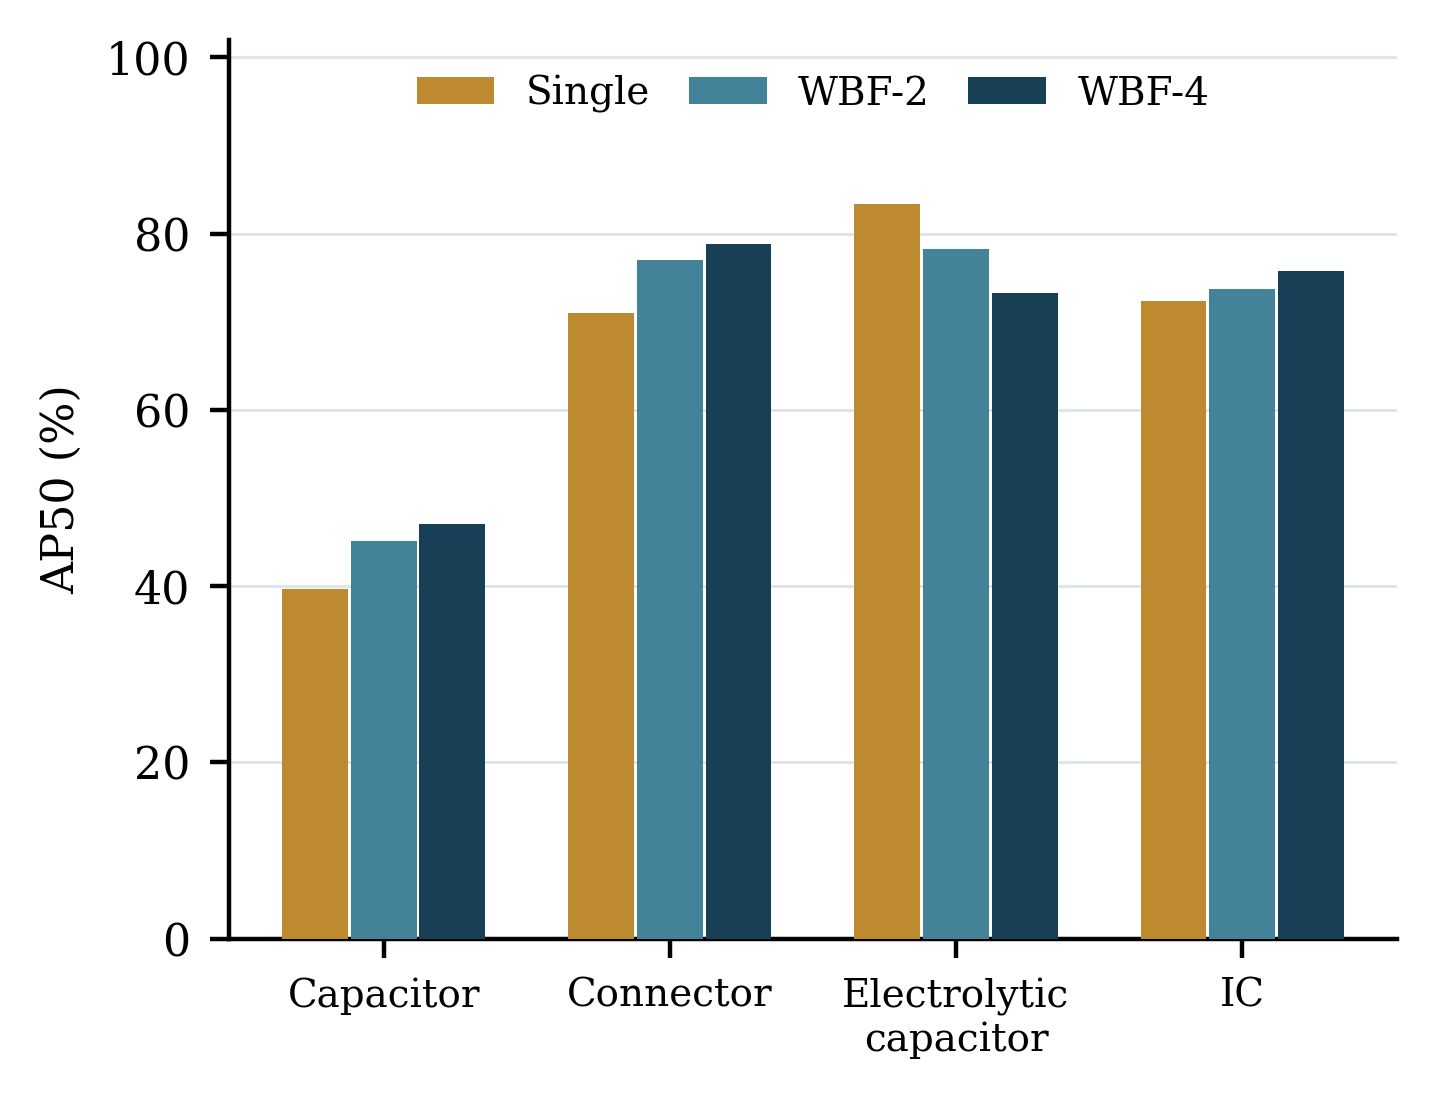
\includegraphics[width=\columnwidth]{figures/native_class_ap.png}
\caption{Per-class AP50 for the crop-trained single model and the fixed WBF ensembles on the same legacy exports. Fusion helps several categories but lowers electrolytic-capacitor AP relative to the crop specialist.}
\label{fig:classes}\end{figure}

\paragraph{Accuracy and deployment cost.}
Two-model and four-model WBF attain 68.49\% and 68.74\% AP50. Relative to the best
selected single checkpoint, the gains are 1.93 and 2.18 percentage points.
Four-model WBF also reaches 47.66\% AP50:95 and 57.75\% pooled F1. Its capacitor
and IC AP50 increase to 47.04\% and 75.77\%, respectively. The improvement is
not uniform: the four-model electrolytic score falls to 73.31\%.

The crop specialist requires 11.11~ms per image (89.99 FPS), versus 47.94~ms
(20.86 FPS) for two-model WBF and 115.97~ms (8.62 FPS) for four-model WBF.
Adding two further models raises AP50 by 0.25 points while increasing latency
by approximately 2.42 times. Thus, the two-model ensemble provides a less costly
ensemble operating point, whereas the crop-trained single model provides the
highest measured throughput among these six configurations. These conclusions
apply to the measured batch-one FP32 H100 pipeline; they do not imply comparable
speed on a different device or precision setting.

\subsection{Qualitative comparison with visible detection differences}
\begin{figure*}[!t]\centering
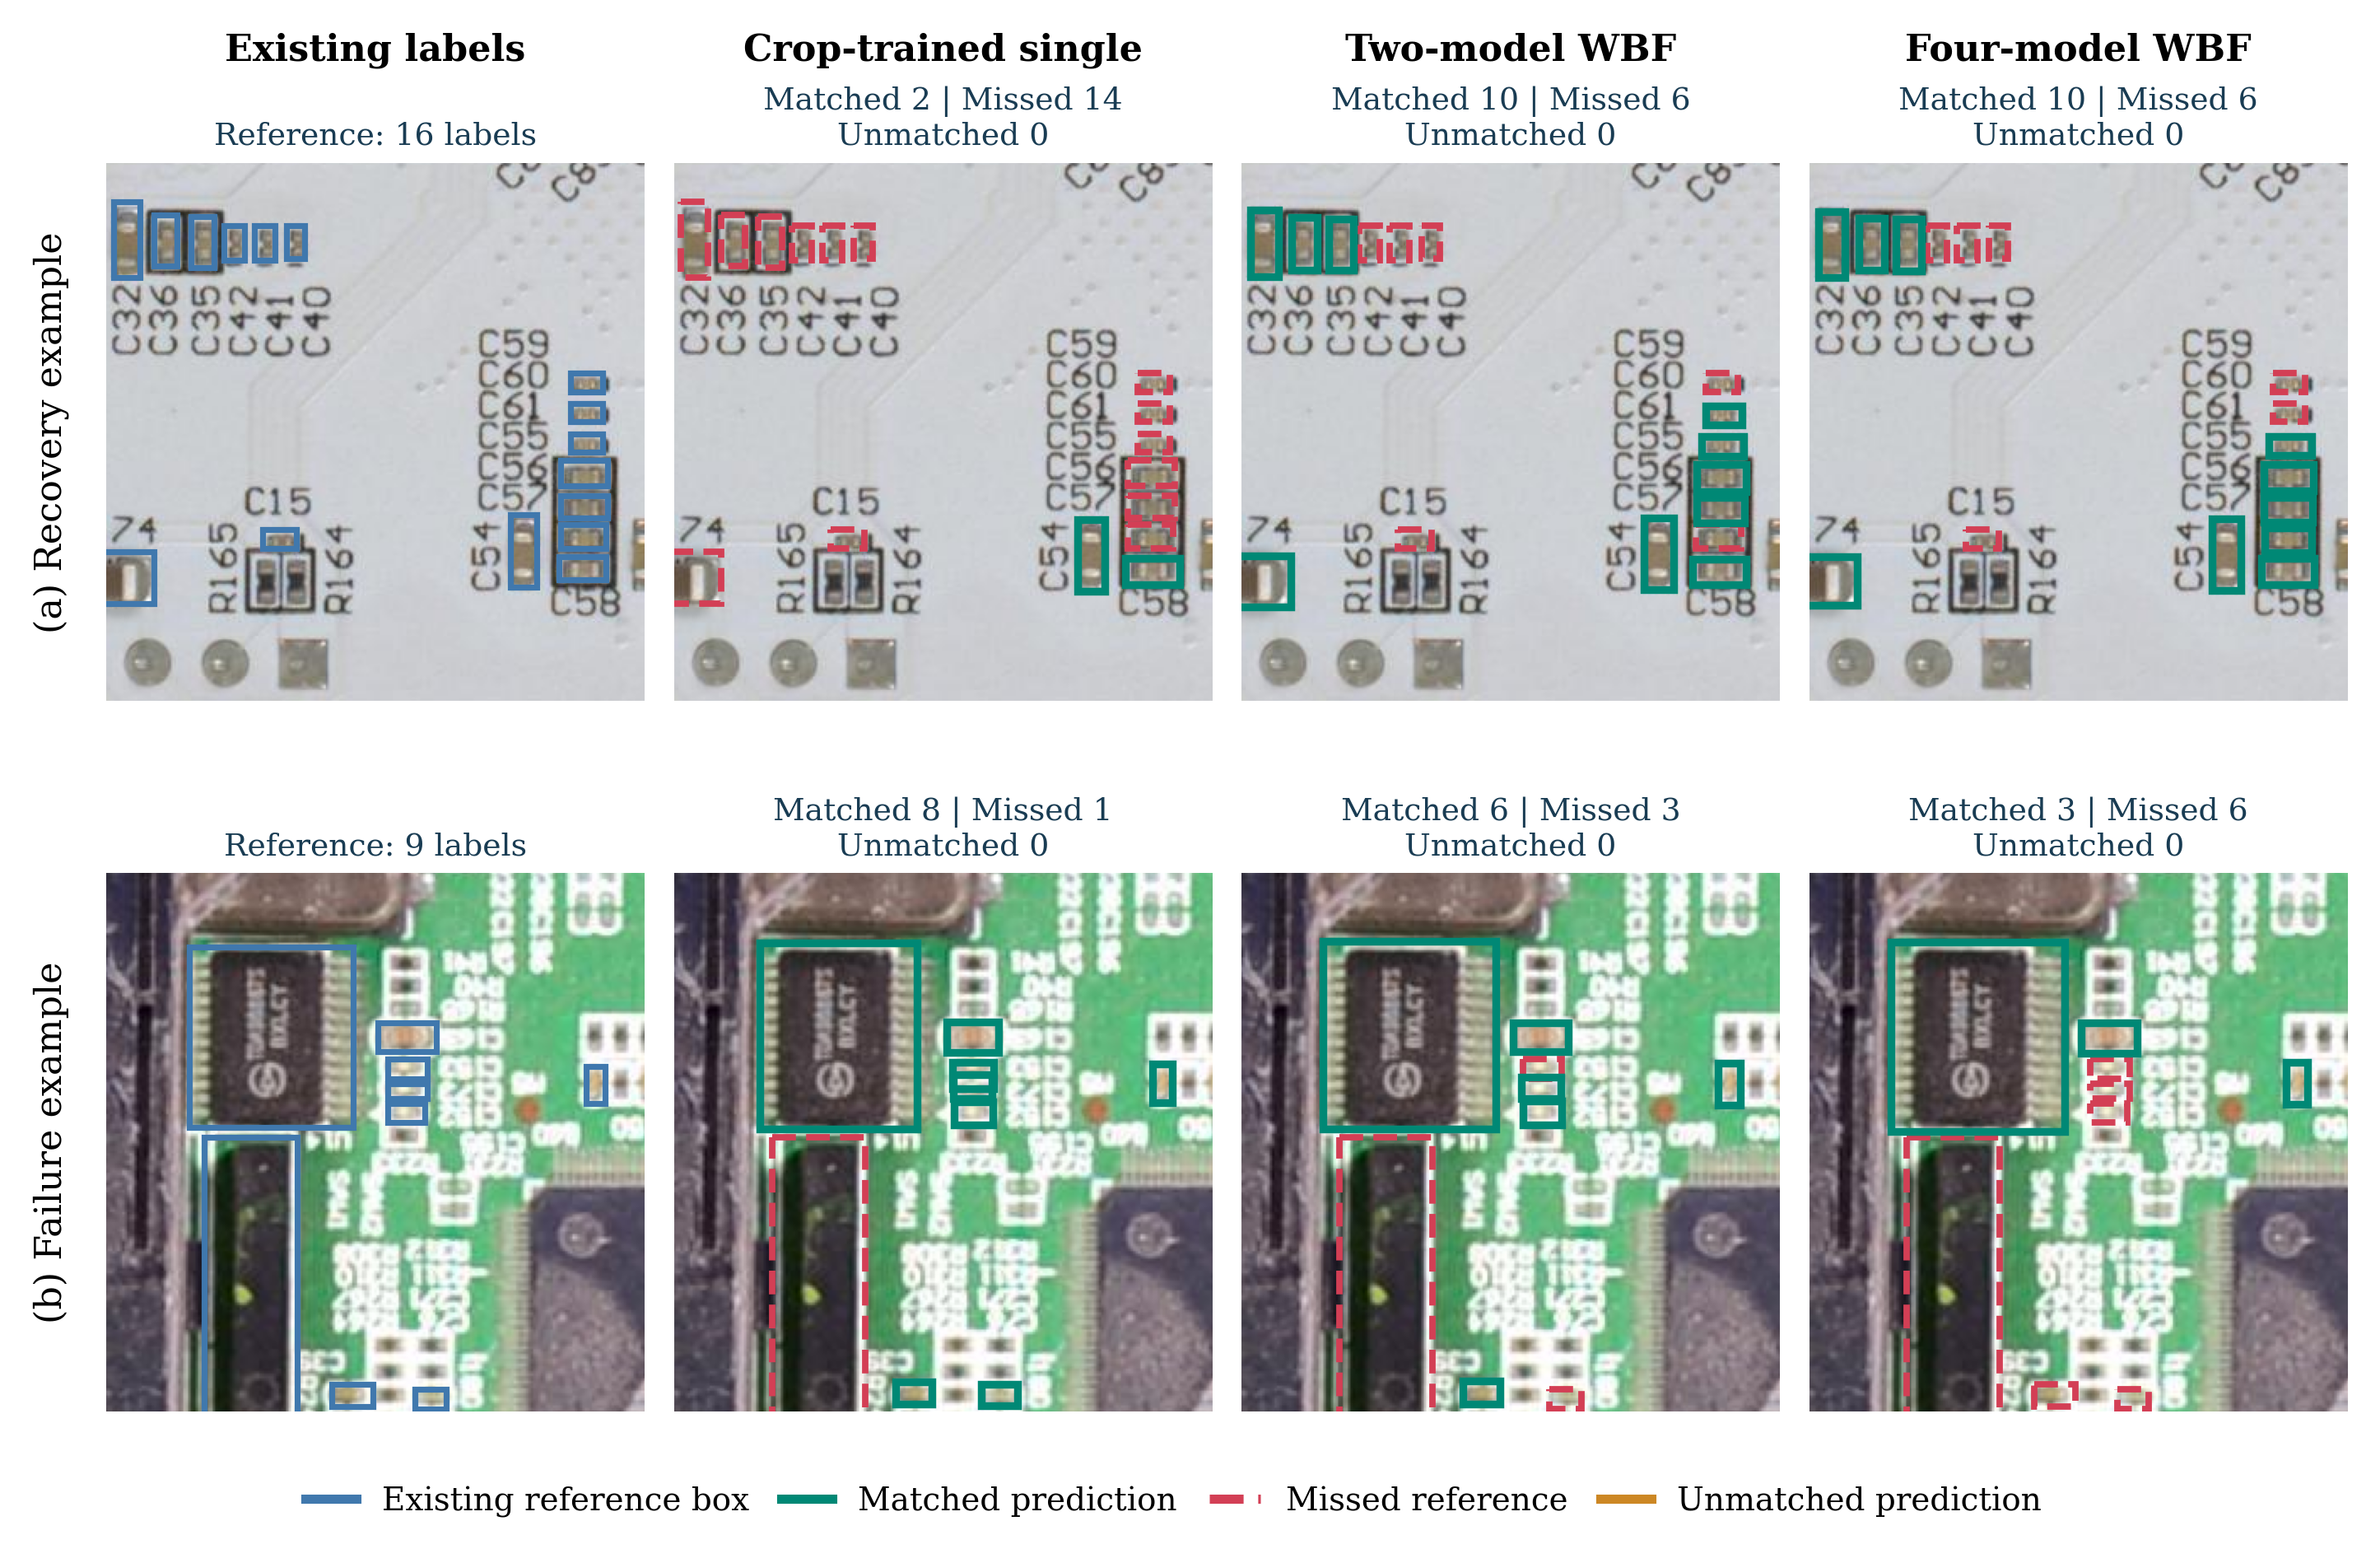
\includegraphics[width=\textwidth]{figures/native_detections.png}
\caption{Enlarged regions showing a recovery case and a reference-score failure case. All columns show identical image pixels within each row. Blue boxes are existing reference annotations; green boxes are matched predictions; dashed red boxes are missed references; orange boxes are unmatched predictions. Counts use local class-aware, one-to-one matching at IoU 0.50 and confidence 0.25; boxes enter a region by their center. Examples were selected after inspecting saved outputs to maximize and minimize the local WBF-4 gain over the single model. They illustrate differences, not their average frequency. Existing annotation omissions can make a real component appear as an unmatched prediction.}
\label{fig:qualitative}\end{figure*}
Figure~\ref{fig:qualitative} presents enlarged dense-component regions for a
direct visual comparison. Each row uses identical image coordinates for the
existing annotations, the crop-trained single model, two-model WBF and four-model
WBF. Matching status, rather than class color alone, makes the
comparison interpretable. No new inference, altered component imagery or
per-model confidence tuning is used: every prediction comes from the frozen
audit caches.

\paragraph{Recovery case.}
The upper row contains a compact cluster of small surface-mounted parts.
The single model misses many reference boxes, while the ensembles recover a
larger subset. This is a local example of complementary predictions improving
coverage. The visible residual dashed boxes also show that fusion does not
recover every component. The display threshold is identical for all pipelines,
but identical numeric thresholds do not imply identical score calibration after
WBF rescaling.

\paragraph{Failure and annotation dependence.}
The lower row deliberately shows an opposing case in which fusion matches fewer
existing labels. Ensemble aggregation can remove low-support predictions or
change localization and confidence, so a local recall improvement is not
guaranteed. Orange boxes denote predictions unmatched to the current reference,
not an expert conclusion that no component exists there. In particular, omitted
or misclassified reference components can create apparent false positives.
Consequently, qualitative comparisons must be interpreted together with the
annotation audit and the aggregate metrics, rather than presented as proof that
an ensemble is uniformly superior.

\subsection{Comparison on the available paper-dataset exports}
\label{sec:papercomparison}
\begin{table*}[!t]
\centering
\caption{Original-label RF100 exports at 640 pixels. Our methods share the same 41-image test split and evaluator (mean $\pm$ sample SD, seeds 0/1/2). P/R/F1 use pooled counts at confidence 0.25 and matching IoU 0.50. Published rows use the authors' protocol and are contextual; a direct improvement claim is unverified.}
\label{tab:paper}\small\setlength{\tabcolsep}{4pt}
\begin{tabular}{lrrrrr}\toprule
Method & $\mathrm{mAP}_{50}$ & $\mathrm{mAP}_{50:95}$ & P & R & F1\\\midrule
\multicolumn{6}{l}{\emph{Our common evaluation protocol (all entries in percent)}}\\
YOLOv8s & $52.34\pm1.38$ & $38.33\pm1.54$ & $61.45\pm1.14$ & $24.04\pm0.46$ & $34.55\pm0.29$ \\
YOLOv12s & $53.61\pm2.39$ & $38.44\pm2.53$ & $62.39\pm3.55$ & $24.58\pm1.55$ & $35.20\pm1.11$ \\
YOLO26s & $49.94\pm1.85$ & $35.03\pm1.12$ & $60.51\pm5.52$ & $24.75\pm1.20$ & $35.04\pm0.31$ \\
AGWD + Dice & $53.23\pm1.40$ & $37.77\pm1.33$ & $58.97\pm4.50$ & $25.18\pm0.41$ & $35.25\pm0.76$ \\
PhysOT & $52.27\pm1.79$ & $37.60\pm1.87$ & $56.87\pm1.82$ & $26.29\pm1.13$ & $35.93\pm0.76$ \\
Crop + AGWD/Dice & $55.08\pm0.89$ & $39.62\pm0.64$ & $59.45\pm2.46$ & $25.84\pm0.99$ & $35.99\pm0.53$ \\
\midrule
\multicolumn{6}{l}{\emph{Published context only~\cite{zhou2026ensemble}; P/R thresholds may differ}}\\
YOLOv8s, best single (Table 4) & 54.04 & -- & 60.6 & 51.8 & --\\
Consensus Top-4, best ensemble (Table 9) & 59.63 & -- & 63.2 & 59.3 & --\\
\bottomrule\end{tabular}\end{table*}

\begin{figure*}[!t]\centering
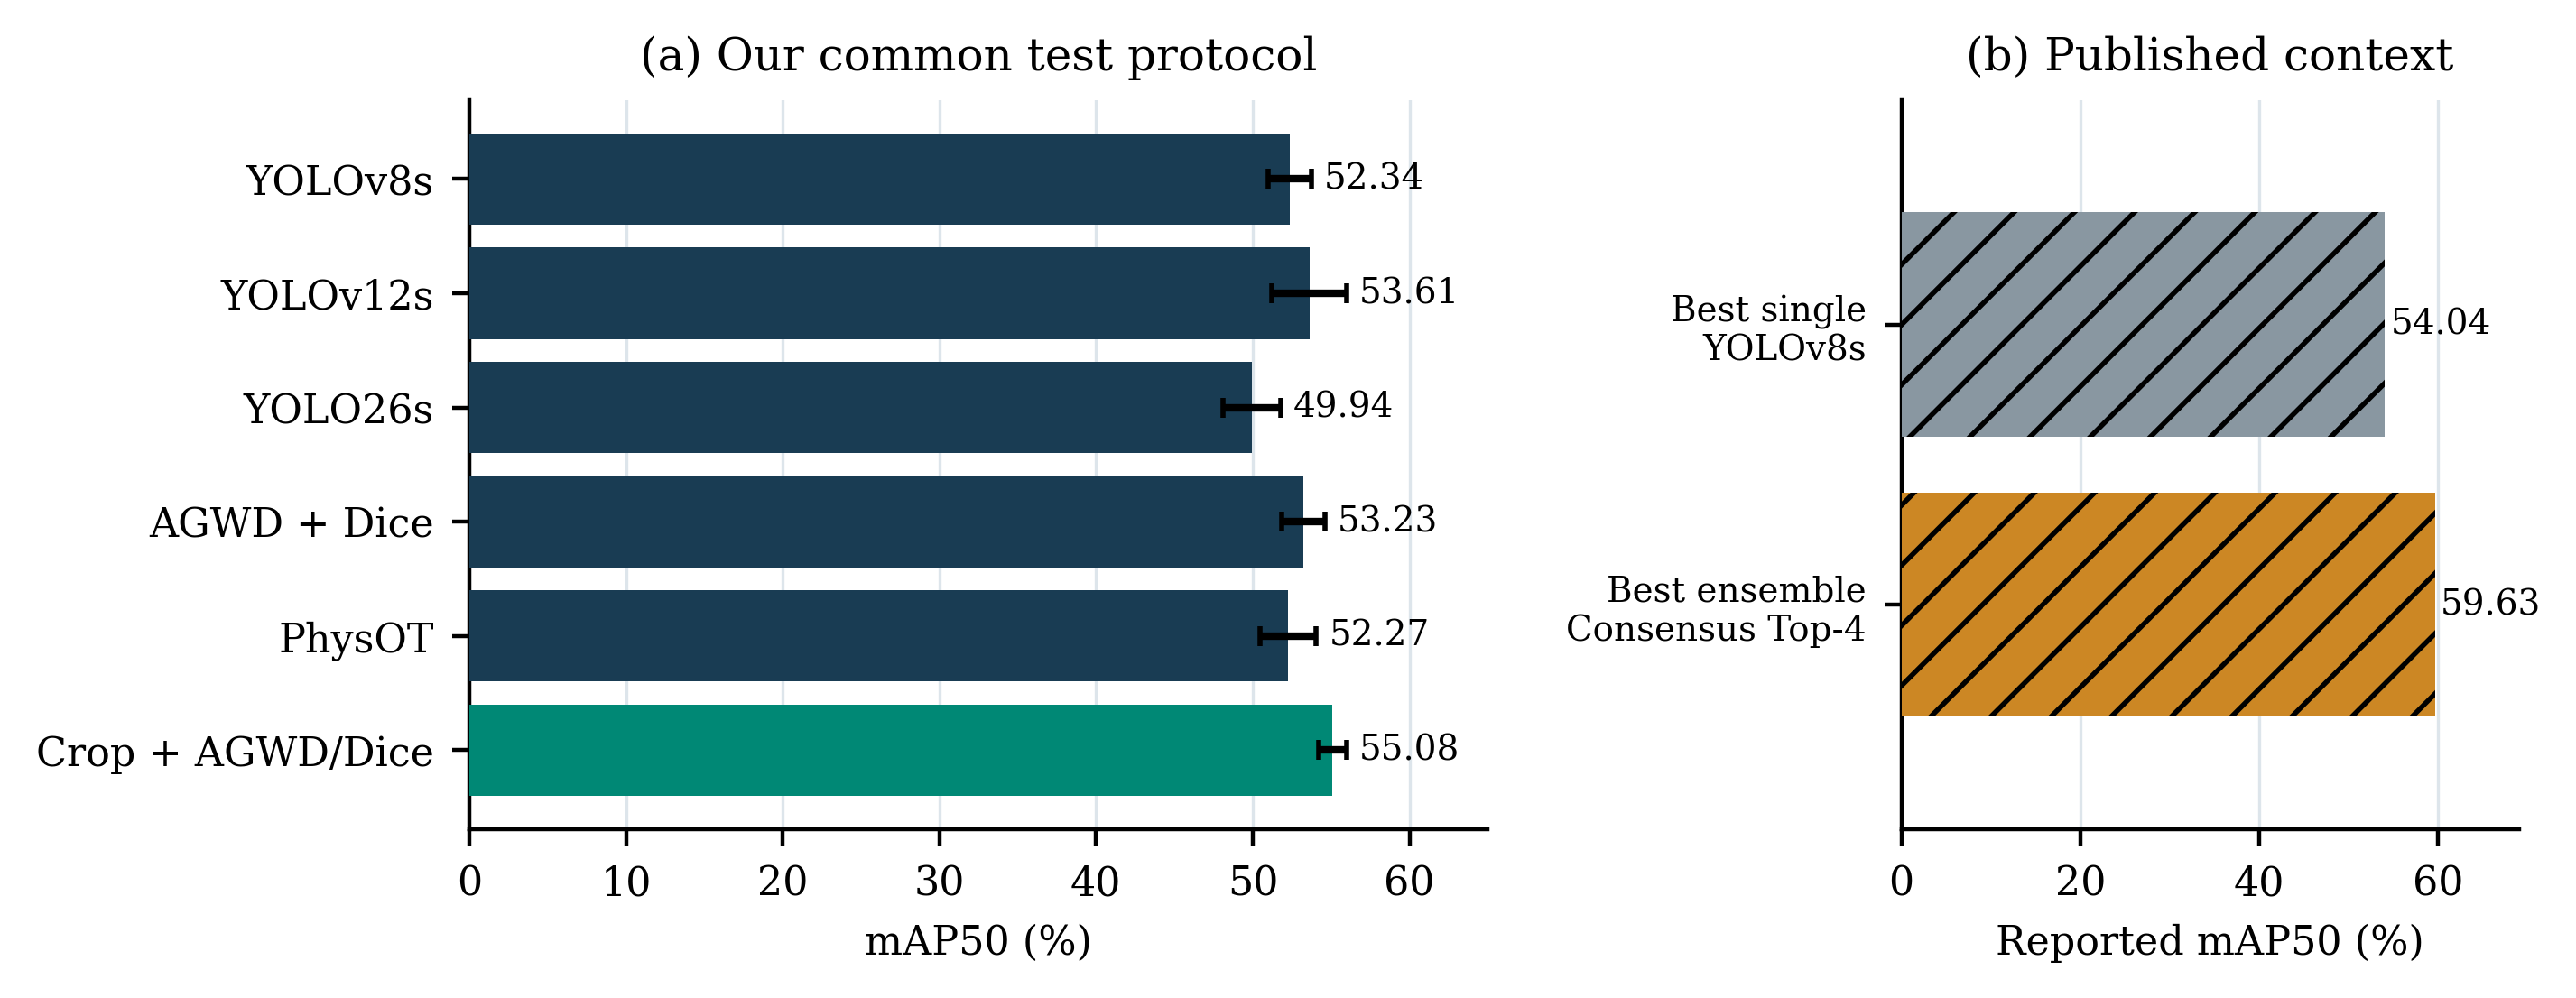
\includegraphics[width=\textwidth]{figures/paper_comparison.png}
\caption{Original-label 640-pixel results and the published reference. Left: our common-protocol mean AP50 with sample SD across three seeds. Right: Zhou and Agaian's reported best individual and ensemble scores~\cite{zhou2026ensemble}. The separate panels indicate distinct evaluation protocols; they are not a certified common leaderboard.}
\label{fig:papercomparison}\end{figure*}
The crop-trained AGWD--Dice model obtains $55.08\pm0.89$\% AP50 and
$39.62\pm0.64$\% AP50:95 under our common evaluator
(Table~\ref{tab:paper}). Relative to our retrained YOLO26s control, the mean gains
are 5.14 and 4.59 percentage points. Relative to our retrained YOLOv8s, the AP50
gain is 2.73 points; relative to YOLOv12s, it is 1.47 points. These are observed
mean differences across three seeds. Sample SD describes run-to-run variability,
not a confidence interval or evidence of statistical significance.

\paragraph{Published best single model and ensemble.}
Zhou and Agaian~\cite{zhou2026ensemble} report 54.04\% AP50 for YOLOv8s, their best
individual model, and 59.63\% for Consensus Top-4, their best ensemble
(Figure~\ref{fig:papercomparison}). Our crop model's mean is numerically 1.04
points above the reported single model and 4.55 points below the reported
ensemble. The latter comparison does not support a claim of beating the
published best ensemble. Our native 1280-pixel WBF results must not be substituted
into this 640-pixel original-label comparison.

Exact protocol equivalence remains unresolved. For example, our available
validation export contains 1,032 IC boxes, while their class table lists 1,026.
Published descriptions and public evaluator paths also differ in split and AP
settings. Using images from the same source dataset alone does not establish
identical annotations, evaluation images, confidence filtering or detection
limits. The published rows are therefore reported as contextual values, while
our own controls provide the directly comparable measurements. Cross-hardware
speedups against the authors' machine are not claimed.

\begin{figure*}[!t]\centering
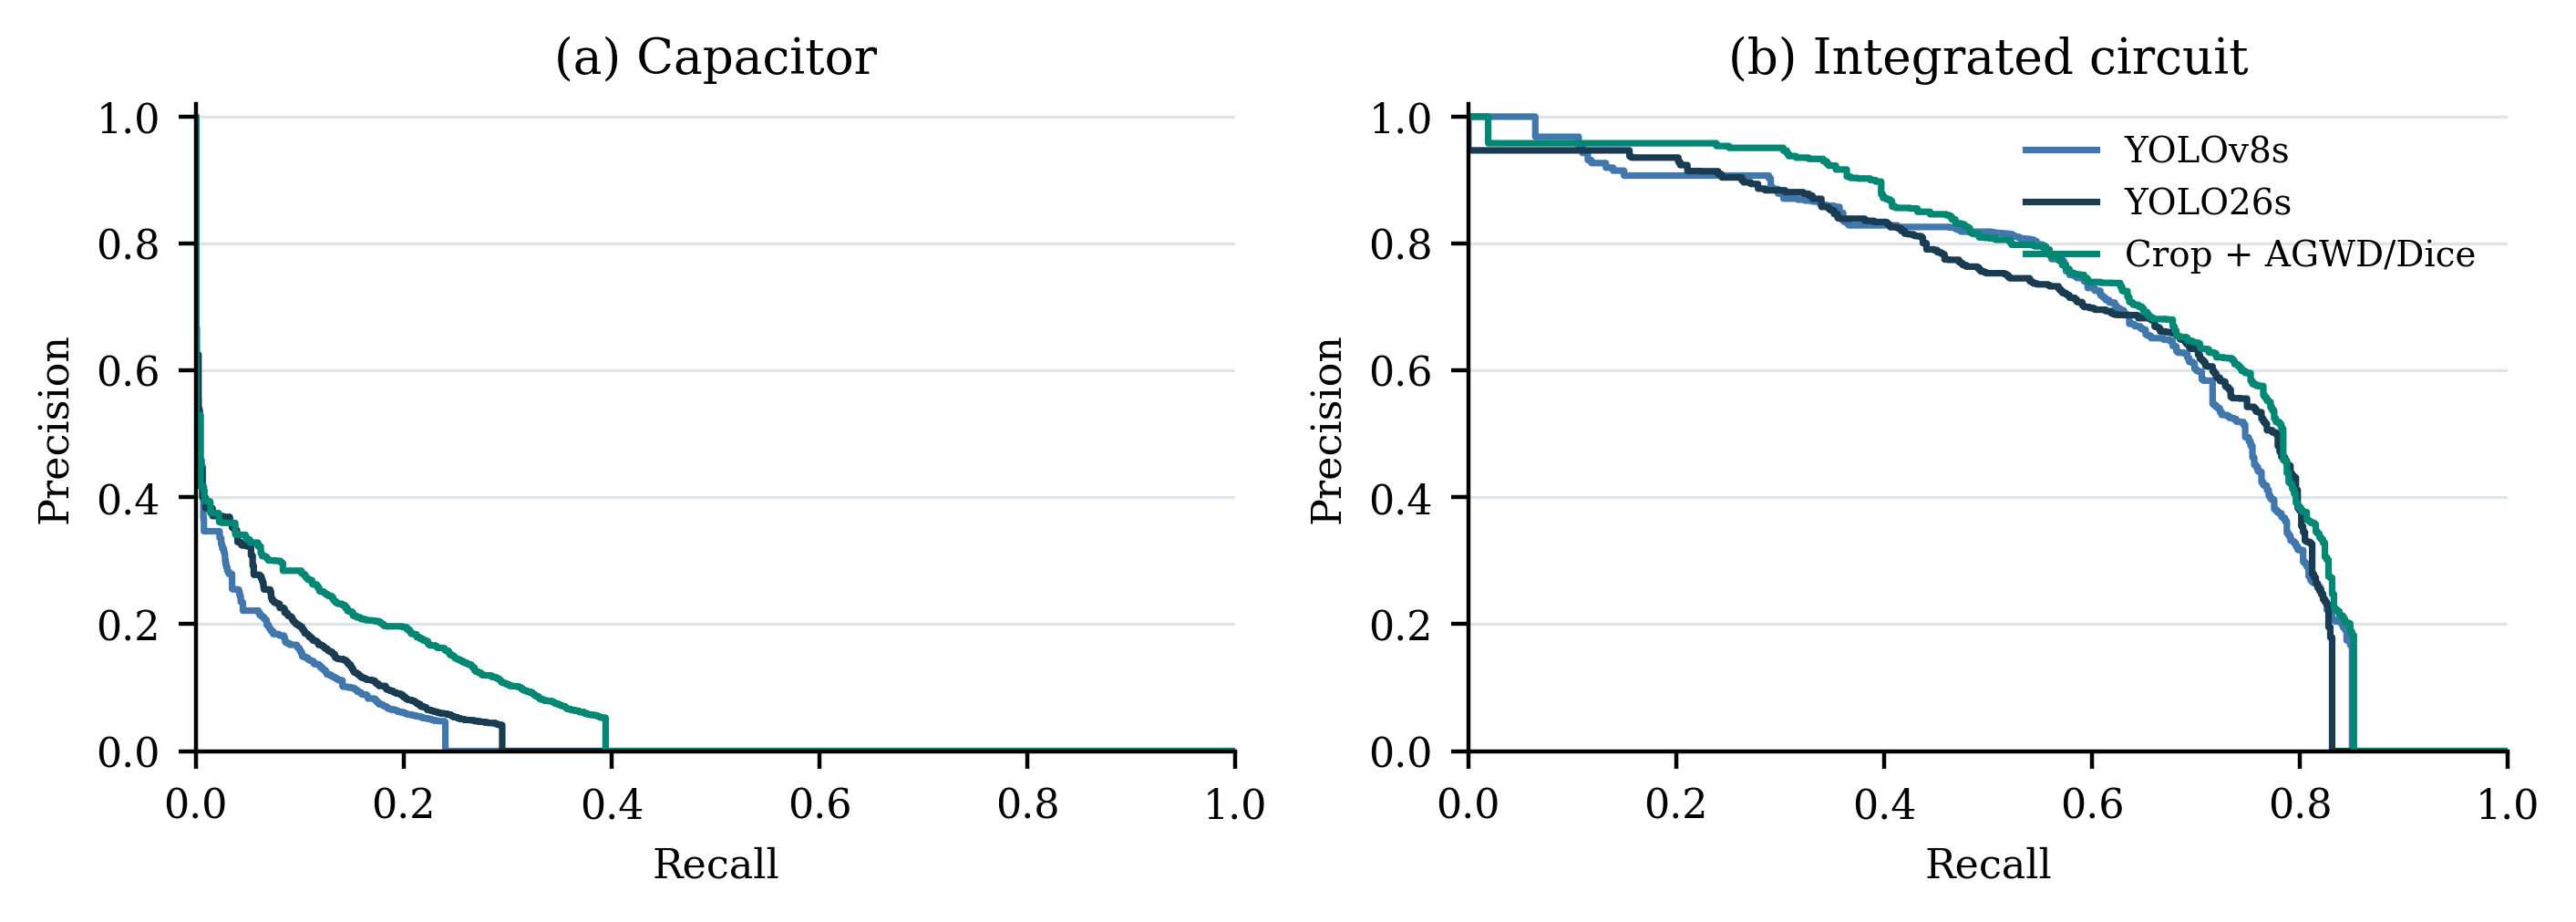
\includegraphics[width=\textwidth]{figures/paper_pr_curves.png}
\caption{Confidence-ranked precision--recall envelopes for capacitor and IC detection on the original-label test exports. These are saved seed-0 predictions, independently checked against the recorded AP50, rather than averaged curves. All three seeds enter Table~\ref{tab:paper}. The large class difference also illustrates why overall mAP alone is insufficient.}
\label{fig:pr}\end{figure*}
The curves in Figure~\ref{fig:pr} provide a class-specific view of the original-label
study. Capacitor detection remains substantially more difficult than IC detection.
The benchmark is also inherited from earlier development, and a filename audit
finds three view-name aliases shared across splits. Thus, this study supports a
controlled comparison on the available exports, rather than certification of
performance on previously unseen physical boards.

\subsection{Hyperparameter sensitivity and supporting ablations}
\begin{table}[!t]
\centering\caption{Historical AGWD--Squared-Dice configurations on legacy test labels. Seed 0 only; percentages. These are development observations, not independent parameter-selection evidence.}
\label{tab:sweep}\footnotesize\setlength{\tabcolsep}{3pt}
\begin{tabular}{rrlrrr}\toprule
$\lambda$ & $\epsilon$ & Stage weights & AP50 & AP50:95 & Cap AP50\\\midrule
0.2 & 0.01 & Uniform & 64.93 & 44.95 & 42.95 \\
0.35 & 0.01 & Uniform & 64.80 & 45.76 & 41.37 \\
0.5 & 0.01 & Uniform & 65.78 & 44.37 & 43.59 \\
0.5 & 0.1 & Uniform & 61.88 & 41.87 & 39.93 \\
0.5 & 0.01 & 0.5/0.3/0.2 & 62.47 & 43.10 & 37.91 \\
1 & 0.01 & 0.5/0.3/0.2 & 61.54 & 41.35 & 38.46 \\
0.5 & 1 & 0.5/0.3/0.2 & 64.87 & 43.97 & 39.15 \\
\bottomrule\end{tabular}\end{table}

\begin{table}[!t]\centering
\caption{Separate repeated-seed native study: mean $\pm$ sample SD, three seeds, no extra online augmentation. Rectangular batch-8 evaluation differs from Table~\ref{tab:native}. Accuracy entries are percentages.}
\label{tab:controlled}\footnotesize\setlength{\tabcolsep}{3pt}
\begin{tabular}{lrrr}\toprule
Recipe ($\lambda$) & AP50 & AP50:95 & Cap AP50\\\midrule
YOLO26s control & $59.47\pm2.45$ & $40.75\pm2.19$ & $33.34\pm3.02$ \\
Squared-Dice, 0.50 & $58.00\pm2.41$ & $42.49\pm2.48$ & $29.30\pm2.15$ \\
AGWD + Dice, 0.35 & $59.56\pm2.61$ & $38.91\pm0.43$ & $32.41\pm2.21$ \\
AGWD + Dice, 0.50 & $58.02\pm1.46$ & $40.70\pm1.05$ & $30.10\pm2.61$ \\
\bottomrule\end{tabular}\end{table}

Squared-Dice is controlled by more than its loss coefficient. In the recorded
experiments, $\lambda$ scales the auxiliary classification term, $\epsilon$
is its smoothing constant, and the stage weights determine the relative
contribution of pyramid levels. The normalized stage aggregation is
\begin{equation}
\mathcal{L}_{\mathrm{aux}}=\frac{\sum_s w_s\mathcal{L}_{\mathrm{SD},s}}{\sum_s w_s},
\qquad
\mathcal{L}_{\mathrm{cls}}=\mathcal{L}_{\mathrm{BCE}}+\lambda\mathcal{L}_{\mathrm{aux}}.
\end{equation}
Uniform stage weights and $(0.5,0.3,0.2)$ weighting are both present in the saved
launch records. Table~\ref{tab:sweep} reports all seven historical configurations,
including settings that performed worse.

\begin{figure*}[!t]\centering
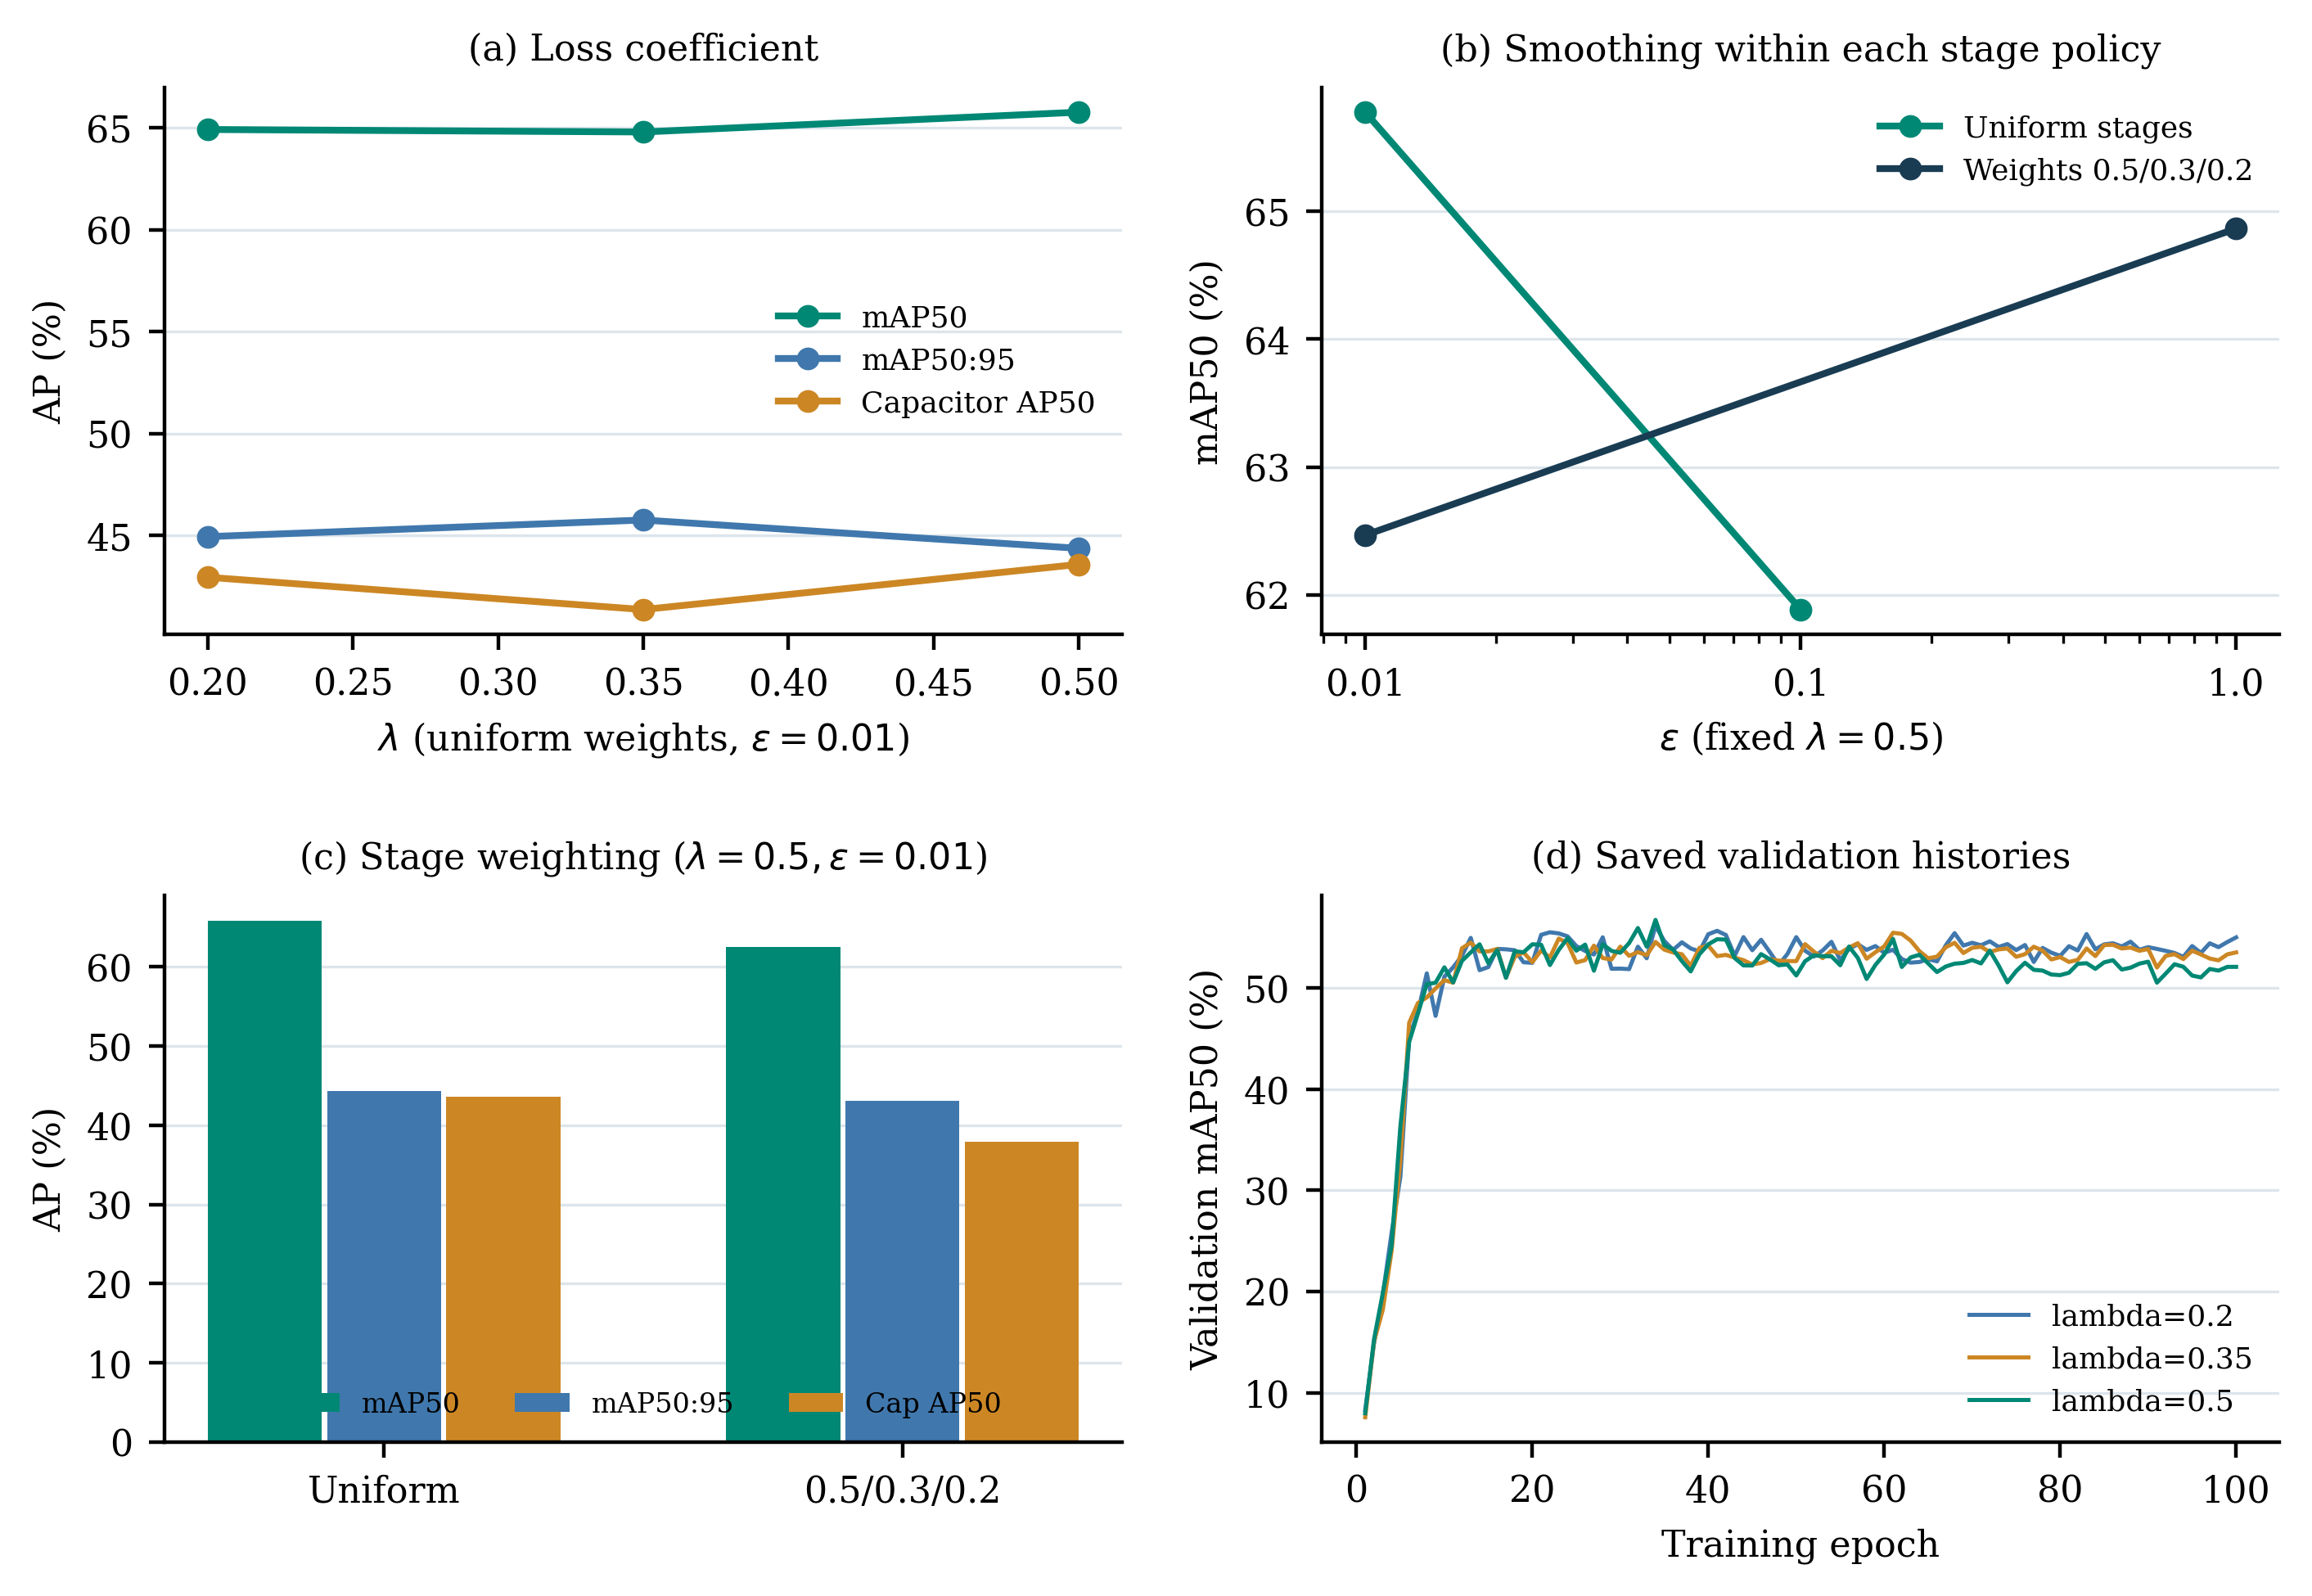
\includegraphics[width=\textwidth]{figures/hyperparameter_sensitivity.png}
\caption{Historical AGWD--Squared-Dice sensitivity. (a) Uniform-stage coefficient sweep at fixed smoothing 0.01. (b) Smoothing comparisons within each stage policy at fixed coefficient 0.5. (c) Stage weighting at fixed coefficient 0.5 and smoothing 0.01. (d) Unsmoothed saved validation histories for the three uniform-stage coefficient runs. Only recorded configurations are shown; connecting lines guide the eye. These are seed-0 development observations, with legacy split and annotation limitations.}
\label{fig:sensitivity}\end{figure*}

\paragraph{Coefficient sweep.}
With uniform stages and $\epsilon=0.01$, the tested coefficients 0.20, 0.35 and
0.50 give AP50 values of 64.93\%, 64.80\% and 65.78\%, respectively. The highest
AP50:95 among these runs occurs at 0.35 (45.76\%), whereas the highest capacitor
AP50 occurs at 0.50 (43.59\%). The preferred setting therefore depends on the
metric. Importantly, the saved $\lambda=1.0$ run also changes the stage weights;
it is not an additional point in the isolated uniform-stage coefficient curve.

\paragraph{Smoothing and stage weighting.}
At $\lambda=0.5$ with uniform stages, changing smoothing from 0.01 to 0.1 lowers
AP50 from 65.78\% to 61.88\%. At smoothing 0.01, using stage weights
$(0.5,0.3,0.2)$ gives 62.47\%, below the uniform-stage result. Under that weighted
stage policy, smoothing 1.0 gives 64.87\%. Smoothing and stage weighting must
therefore be examined within matched settings; combining all such runs into a
single smoothing curve would confound two changes. The historical uniform
$\lambda=0.5,\epsilon=0.01$ checkpoint remains a useful selected configuration,
not a demonstrated universal optimum. Its earlier batch-8 test score also must
not replace its separately measured square batch-one champion-audit score.

\paragraph{Repeated-seed loss controls.}
Table~\ref{tab:controlled} provides a separate completed native study using no
extra online augmentation and rectangular batch-8 evaluation. AGWD--Dice with
$\lambda=0.35$ gives $59.56\pm2.61$\% AP50, versus $58.02\pm1.46$\% at
$\lambda=0.50$. However, the standard YOLO26s control gives
$59.47\pm2.45$\% AP50 and higher AP50:95 than either combined-loss setting.
These results limit any claim that adding the proposed loss terms always
improves detection. The differences between this study and the older sweeps
also show why training recipes and evaluator settings must remain explicit.

AGWD's pixel-length/area scales are rescaled from 12.8 pixels/576 pixels$^2$
at input size 1280 to 6.4 pixels/144 pixels$^2$ at size 640; this is not a
threshold sweep. Historical test-guided development does not replace independent
final evaluation.

\twocolumn[{\begin{minipage}{\textwidth}
\subsection{Dataset taxonomy and annotation-quality analysis}
\subsubsection{Class-name consolidation}
\centering
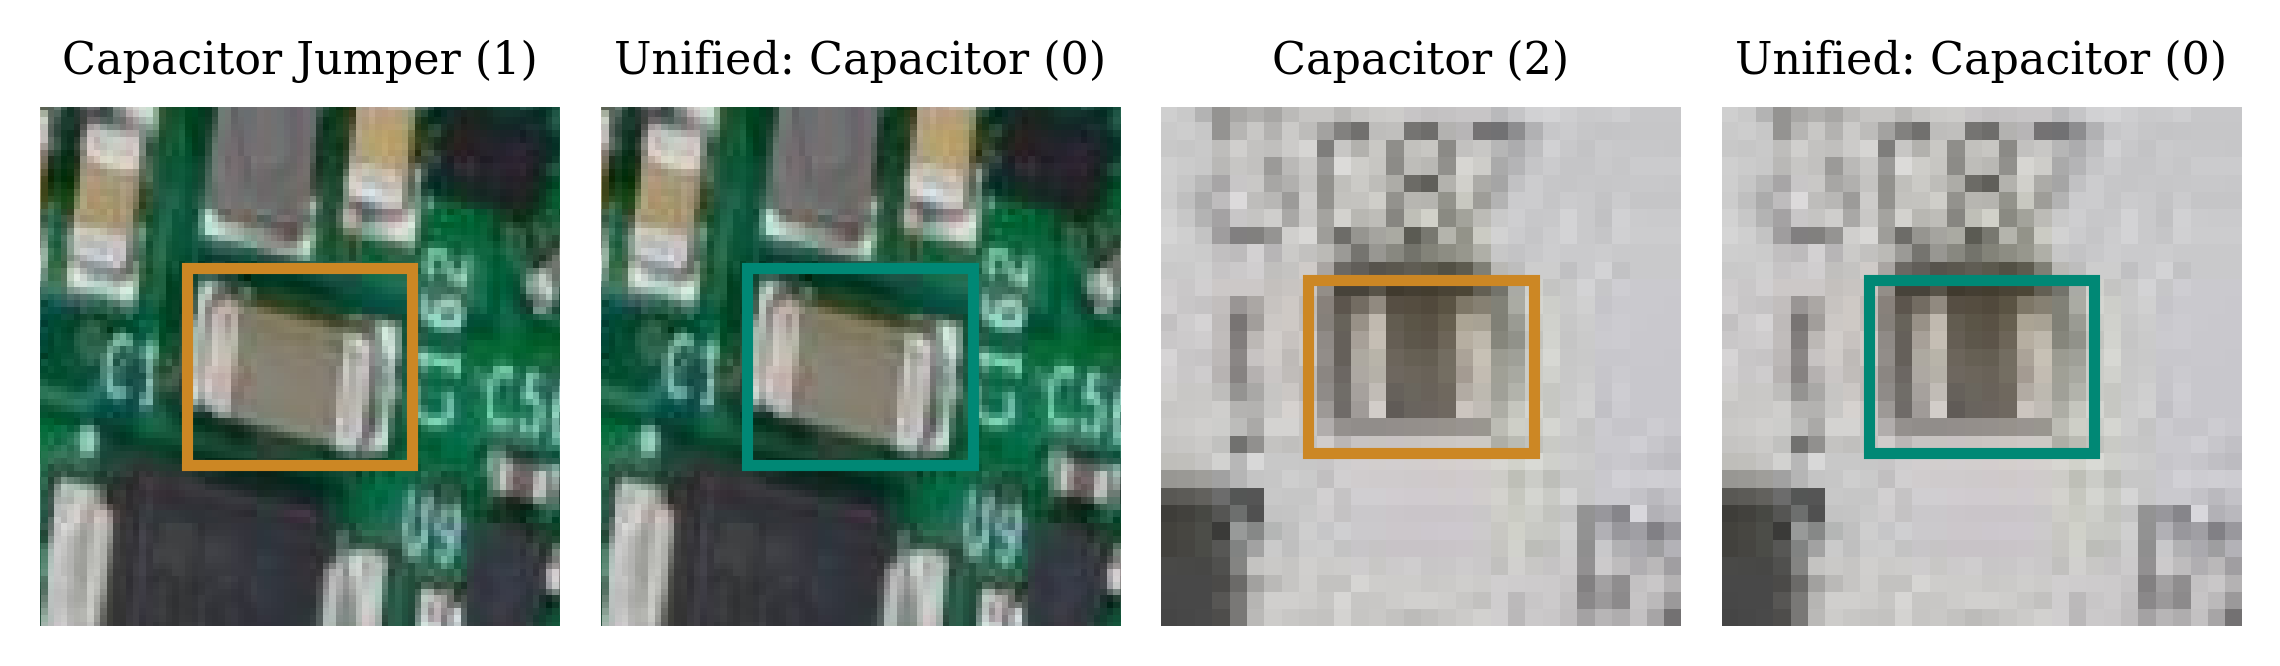
\includegraphics[width=\textwidth]{figures/taxonomy_consolidation.png}
\captionof{figure}{Original-label examples illustrating the main pipeline's capacitor-name consolidation. A source class-1 \emph{Capacitor Jumper} example and a source class-2 \emph{Capacitor} example map to canonical class 0. Each before/after pair uses the same image and coordinates. This is a task-level taxonomy decision, not proof that every source instance is correctly annotated. The original-label paper-comparison track deliberately excludes source class 1.}
\label{fig:taxonomy}
\end{minipage}\vspace{10pt}}]

The raw RF100 export defines 23 class names. The main four-class pipeline
consolidates source \emph{Capacitor Jumper} (ID 1) and \emph{Capacitor} (ID 2)
into canonical \emph{Capacitor} (ID 0). It also maps \emph{IC} (ID 9) and
\emph{iC} (ID 22) into canonical \emph{IC} (ID 3). Connector and electrolytic
capacitor labels map to IDs 1 and 2. Other source categories are outside this
four-class detection task. Figure~\ref{fig:taxonomy} shows two concrete source
annotations alongside their canonical names.

\begin{table}[!t]\centering
\caption{Canonical mapping in the main dataset builder. Counts refer to source annotations across exported splits, not independent physical parts.}
\label{tab:taxonomy}\footnotesize\setlength{\tabcolsep}{2.8pt}
\begin{tabular}{lrl}\toprule
Source class & Source boxes & Main canonical class\\\midrule
Capacitor Jumper (1) & 19,034 & Capacitor (0)\\
Capacitor (2) & 32,564 & Capacitor (0)\\
Connector (4) & 4,558 & Connector (1)\\
Electrolytic Capacitor (7) & 856 & Electrolytic Cap. (2)\\
IC (9) & 7,604 & IC (3)\\
iC (22) & 0 & IC (3)\\\bottomrule
\end{tabular}\end{table}

The capitalization alias is supported by the schema and mapping code, but the
checked source export contains zero ID-22 instances. We therefore do not
attribute an observed annotation improvement or accuracy gain to that alias.
The capacitor grouping has affected instances, but name consolidation alone
does not validate their component identity. Some source annotations are
visually inconsistent, so instance-level review remains necessary. In particular,
this consolidation is distinct from the later decision to label clearly
identifiable electrolytic capacitors consistently as class 2. Ambiguous tiny
SMD parts retain their existing labels rather than receiving guessed identities.

The original-label comparison in Section~\ref{sec:papercomparison} intentionally uses only original
IDs 2, 4, 7 and 9. It excludes Capacitor Jumper and imports no cleaned boxes.
This distinction preserves the provenance of the paper-dataset study and
prevents a taxonomy change from being presented as an algorithmic gain.

\subsubsection{Reviewed corrections and split isolation}
\begin{table}[!t]
\centering
\caption{Recorded r3 edits and quarantined exports. Counts include resized or
transformed views, rather than independent physical components.}
\label{tab:review}
\footnotesize\setlength{\tabcolsep}{4pt}
\begin{tabular}{lrrrr}
\toprule
Split & Class changes & Added & Removed & Quarantined\\
\midrule
Train & 1454 & 83 & 21 & 56\\
Validation & 100 & 12 & 0 & 2\\
Test & 204 & 0 & 4 & 0\\
\midrule
Total & 1758 & 95 & 25 & 58\\
\bottomrule
\end{tabular}
\end{table}

A later visual audit examined the main legacy source: 672 exports and 64,708
boxes. The resulting r3 candidate records 1,878 edits across 212 exports:
1,758 general-capacitor boxes reclassified as electrolytic, 95 missing boxes
added, and 25 boxes on unpopulated footprints removed. Existing coordinates
are retained for the class-only corrections. The additions represent 27
reference physical components across five photographed views and their
registered variants; 95 is not the count of independent added parts.
Table~\ref{tab:review} separates edits by split.



Feature registration and visual inspection confirmed shared photographs for
ArduinoMega top and DuetWIFI bottom across training/validation, and DuetWIFI top
across training/test. A conservative board-family rule retains each family's
highest-priority existing split (test, then validation, then training) and
quarantines lower-priority exports. No held-out image is moved into training.
This quarantines 56 training and two validation exports across nine families;
quarantining also covers related views beyond the three confirmed photo pairs.
The active candidate has 492 training, 78 validation and 44 test exports, with
60,884 boxes. The source images and labels remain available independently.

\twocolumn[{\begin{minipage}{\textwidth}
\centering
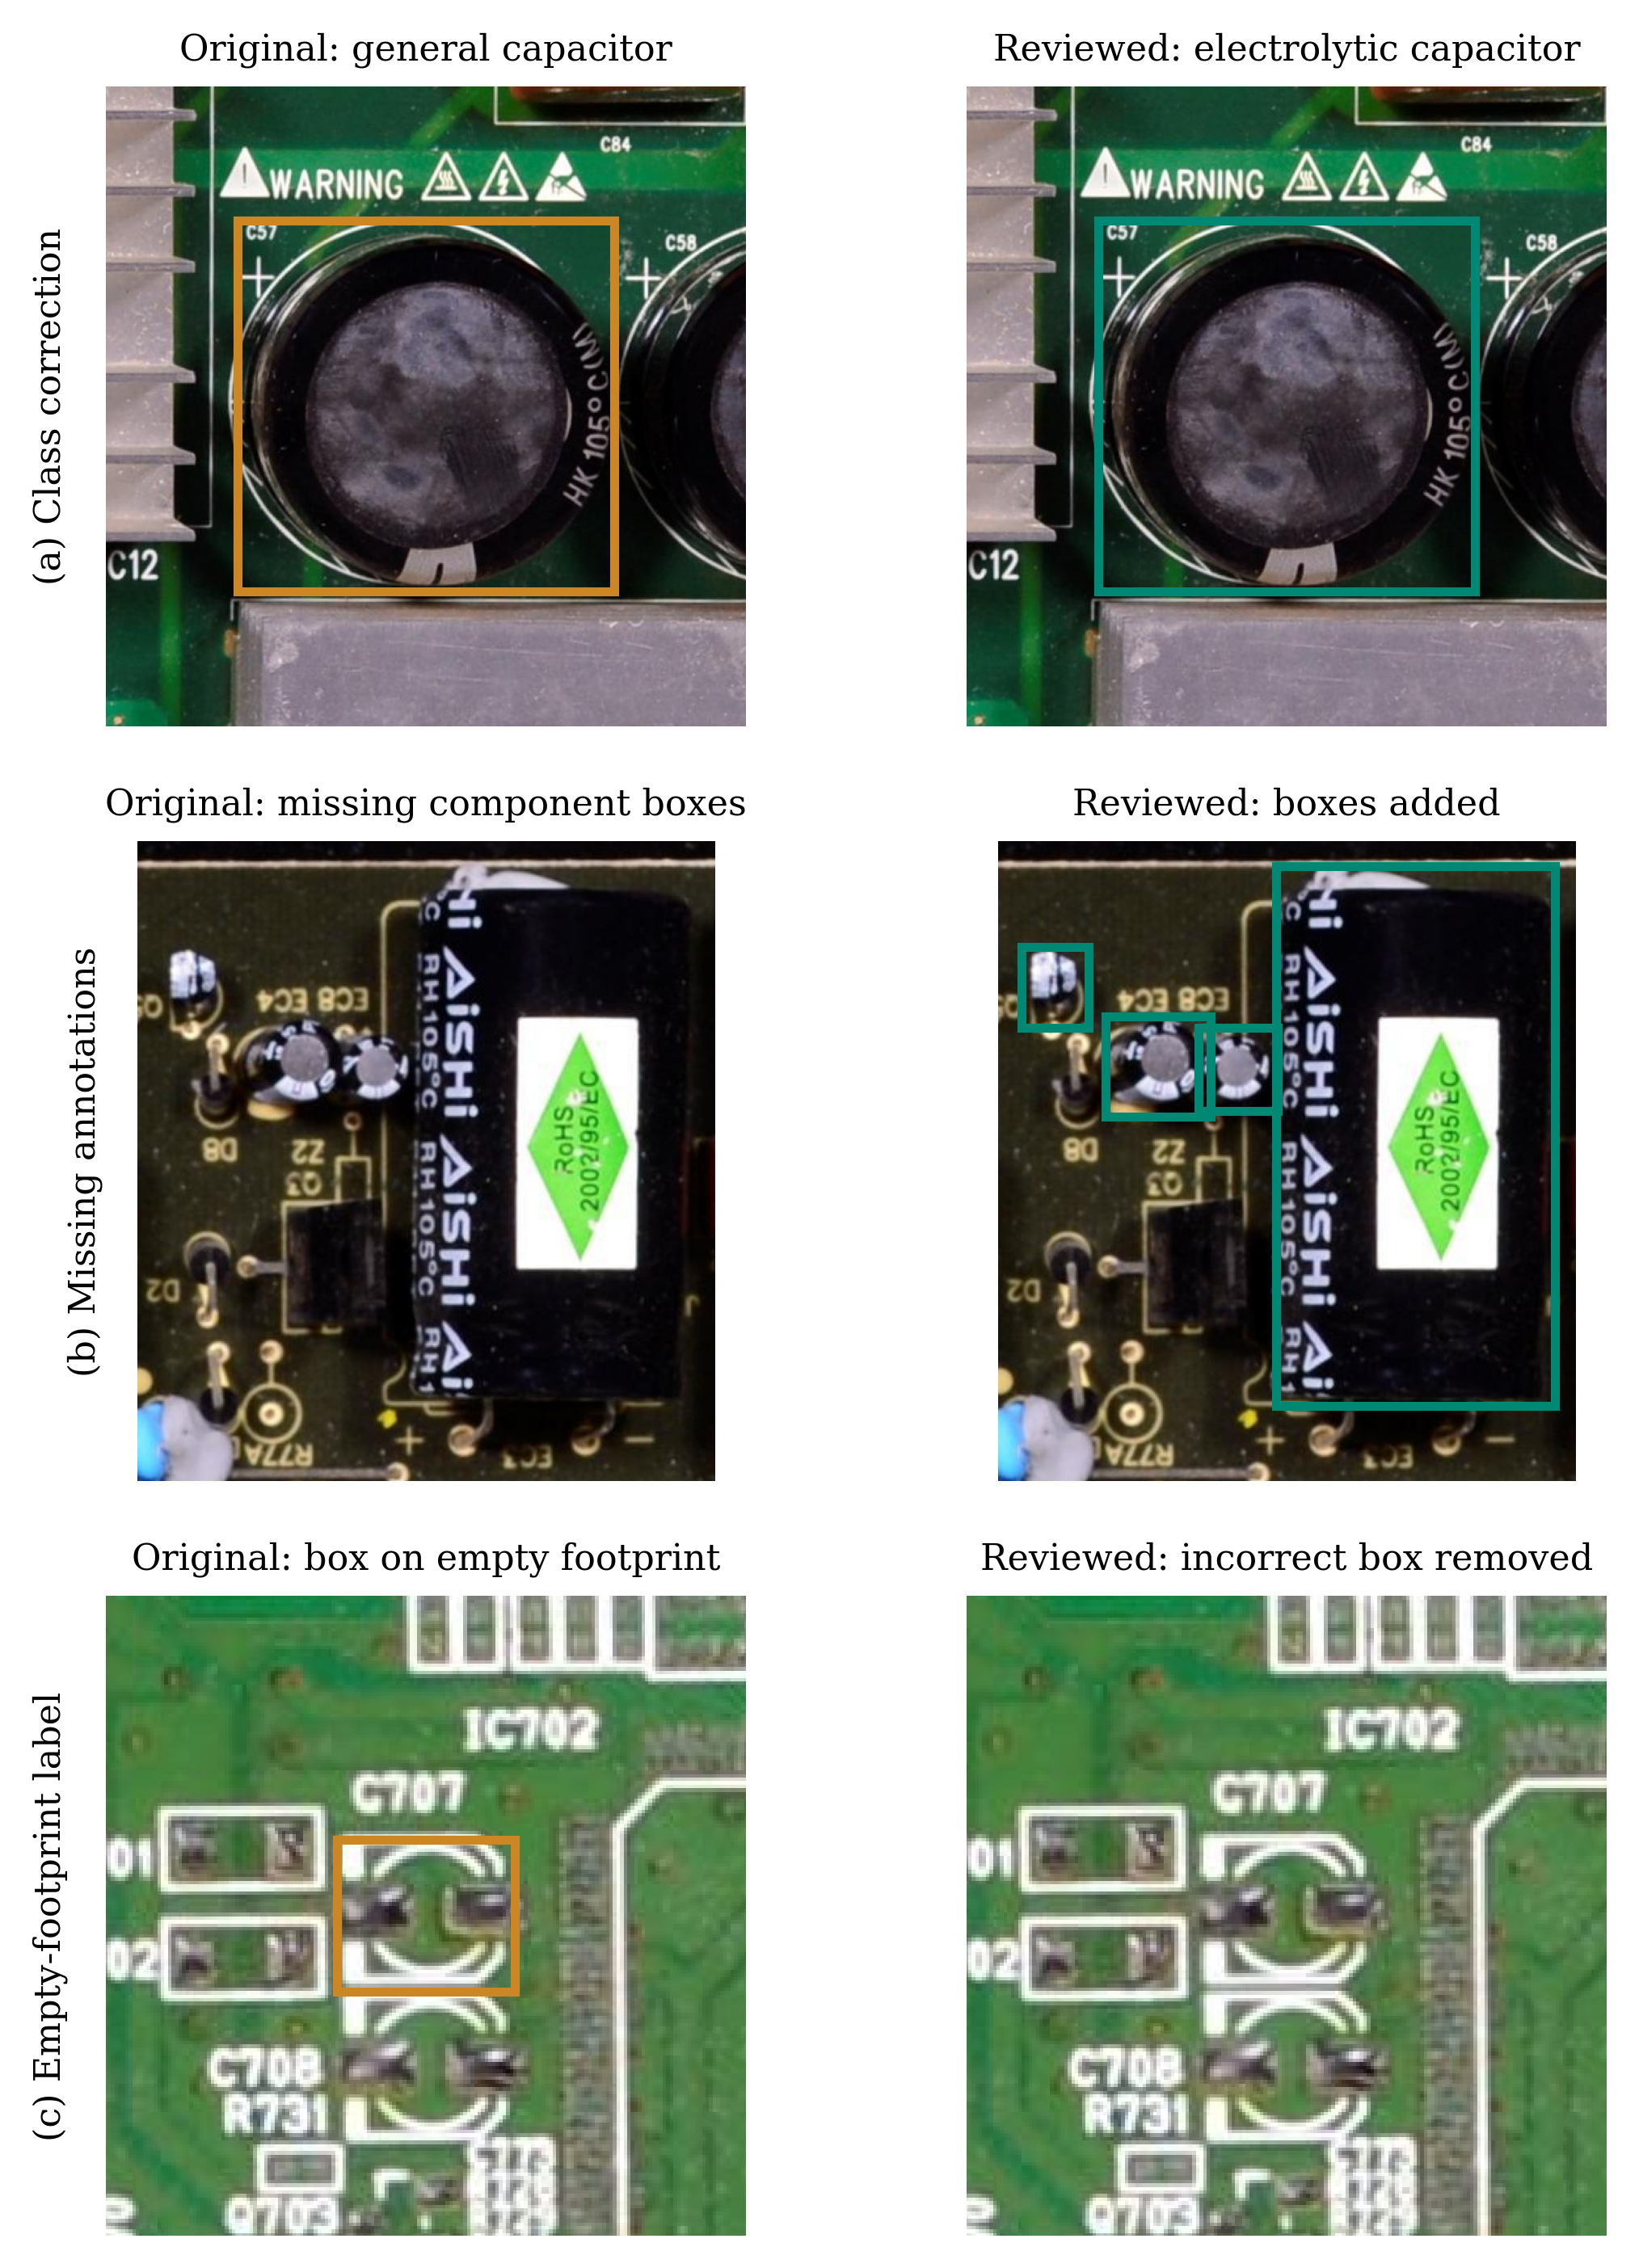
\includegraphics[width=.62\textwidth]{figures/annotation_review.png}
\captionof{figure}{Traced before/after annotation changes. (a) A clearly identifiable electrolytic capacitor receives the consistent class label. (b) Omitted component boxes are added. (c) A box on an unpopulated footprint is removed. Orange denotes the original edited box and green the reviewed box; these overlays are annotations, not detector predictions. Each edit is linked to its source image, label row and visual evidence. Original files are preserved.}
\label{fig:corrections}
\end{minipage}\vspace{10pt}}]


All 672 source images received overview inspection; 554 prioritized component
close-ups and targeted contexts were also examined. This does not verify every
one of the 64,708 original boxes at native resolution. Exhaustive dense-region
review, partial-occlusion policy and final held-out deduplication remain
incomplete. Thirty-six sub-two-pixel source boxes were retained and flagged.
The 1280-pixel dataset name is a training convention: some files have lower
native resolution, and the legacy validation reconstruction upsamples
640-pixel exports without restoring lost visual detail.

These findings explain why annotation quality and split membership require
separate treatment from detector architecture. Missing labels can penalize
valid detections; inconsistent classes can make a correct localization appear
as a class error; shared photographs can inflate apparent generalization.
\newpage
\noindent Figure~\ref{fig:corrections} documents repairs, but no measured post-correction
accuracy gain is claimed in this section. Corrected-data runs and the newer
original-label AGWD/Exp7 runs require their own completed evaluation before
being added to the result tables.
